
\documentclass[letterpaper,11pt]{article}

\usepackage{amsmath}
\usepackage{cite}
\usepackage[margin=1in]{geometry}
\usepackage{graphicx}
\usepackage{tikz}
\usepackage{url}
\usepackage{xspace}

\usetikzlibrary{fit}
\usetikzlibrary{positioning}

\newcommand{\dealii}{\texttt{deal.II}\xspace}
\newcommand{\pforest}{\texttt{p4est}\xspace}

\newcommand{\figref}[1]{Figure~\ref{fig:#1}}

\author{Carsten Burstedde}
\title{Brief \pforest interface schematics}

\begin{document}

\maketitle

\begin{abstract}
We describe the general procedure of using \pforest from application codes.
\pforest is a software library that stores and modifies a forest-of-octrees
refinement structure using distributed (MPI) parallelism.  It expects the
description of the domain as a coarse mesh of conforming hexahedra.
Non-conforming adaptive mesh refinement (AMR), coarsening, and other operations
that modify the forest are implemented as \pforest API functions.  To inform
the application about the refinement structure, several methods are provided
that encode this information.
\end{abstract}

\section{Starting point}

We generally separate the adaptive mesh refinement (AMR) topology from any
numerical information.  The former is stored and modified internally by the
\pforest software library, while an application is free to define the way it
uses this information and arranges numerical and other data.  This document is
inteded to describe the interface by which \pforest transfers mesh information
to the application.

The general, modular AMR pipeline is described in
\cite{BursteddeGhattasStadlerEtAl08}, which is not specific to \pforest but can
in principle be applied to any AMR provider.  The \pforest algorithms and main
interface routines are destribed in \cite{BursteddeWilcoxGhattas11}.
% \cite{IsaacBursteddeGhattas12}
An example usage of \pforest as scalable mesh backend for the general-purpose
finite element software \dealii is described in
\cite{BangerthBursteddeHeisterEtAl11}.  A reference implementation of \pforest
in \texttt{C} can be freely downloaded \cite{Burstedde10} and used and extended
under the GNU General Public License.  This software is best installed
standalone into a dedicated directory, where an application code can then find
the header and library files to compile and link against, respectively.

In this document, we document the three distinct tasks to
\begin{description}
\item[A] create a coarse mesh (\figref{partA}),
\item[B] modify the refinement and partition structure internal to \pforest,
\item[C] and to transfer the mesh information to an application.
\end{description}
Unless indicated otherwise, all operations described below are understood as
MPI collectives, that is, they are called on all processors simultaneously.
Currently, part A needs to be performed redundantly on all processors, which is
acceptable for up to $10^5$--$10^6$ coarse cells (octree roots).  In parts B
and C, runtime and memory are roughly proportional to the number of elements
(octree leaves) on a given processor, independent of the number of octrees.

\begin{figure}
\begin{center}
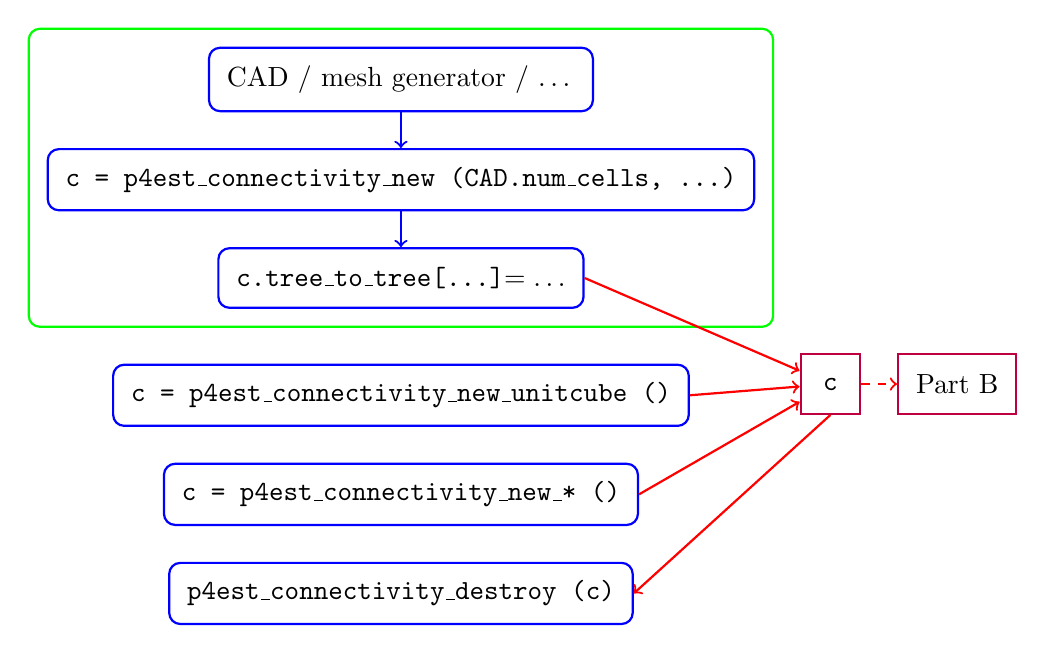
\begin{tikzpicture}[node distance=3ex]

\tikzstyle{group}=[rectangle, rounded corners, thick, draw=green,
  minimum size=5ex, inner sep=1.5ex]
\tikzstyle{action}=[rectangle, rounded corners, thick, draw=blue,
  minimum size=5ex, inner sep=1.5ex]
\tikzstyle{object}=[rectangle, thick, draw=purple,
  minimum size=5ex, inner sep=1.5ex]

\tikzstyle{arrseq}=[->, thick, draw=blue]
\tikzstyle{arrdat}=[->, thick, draw=red]

\node [action] (CAD) {CAD / mesh generator / \ldots};
\node [action, below=of CAD] (connnew) { 
  \texttt{c = p4est\_connectivity\_new (CAD.num\_cells, \ldots)} };
\draw [arrseq] (CAD) -- (connnew);
\node [action, below=of connnew] (connfill) {
  \texttt{c.tree\_to\_tree[\ldots]$ = \ldots$} };
\draw [arrseq] (connnew) -- (connfill);
\node[group, fit=(CAD) (connnew) (connfill)] (cadpipe) {};

\node[action, below=of cadpipe] (newunit) {
  \texttt{c = p4est\_connectivity\_new\_unitcube ()} };

\node[action, below=of newunit] (newstar) {
  \texttt{c = p4est\_connectivity\_new\_* ()} };

\node[object, below right=of cadpipe] (theconn) { \texttt{c} };
\draw[arrdat] (connfill.east) -- (theconn);
\draw[arrdat] (newunit.east) -- (theconn);
\draw[arrdat] (newstar.east) -- (theconn);

\node[object, right=of theconn] (topartb) { Part B };
\draw[arrdat, dashed] (theconn.east) -- (topartb.west);

\node[action, below=of newstar] (conndestroy) {
  \texttt{p4est\_connectivity\_destroy (c)} };
\draw[arrdat] (theconn.south) -- (conndestroy.east);

\end{tikzpicture}
\end{center}
\caption{Part A, creating the coarse mesh connectivity.  The connectivity
  \texttt{c} is a \texttt{C struct} that contains numbers and orientations of
  neighboring coarse cells.  It can be created by translating CAD or mesh data
  file formats or by using one of several \pforest convenience functions.  The
  data format is documented in the big comment blocks in
  \texttt{p4est\_connectivity.h} (2D) and \texttt{p8est\_connectivity.h} (3D).}
\label{fig:partA}
\end{figure}

\bibliographystyle{siam}
\bibliography{ccgo}

\end{document}
